\chapter{Continuité d'Activité et Résilience (ISO 22301)}
\label{chap:continuite}

La gestion d'incident se focalise sur le rétablissement technique. La Continuité d'Activité se concentre sur la survie de l'entreprise et la capacité à maintenir les fonctions vitales pendant une crise majeure.

\section{Présentation : De l'Incident à la Crise Majeure}

\subsection{Définition de la Continuité}

\begin{boxdef}
\textbf{Continuité d'Activité (Business Continuity) :} Capacité stratégique et tactique de l'organisation à planifier et réagir aux incidents et interruptions de service, afin de continuer à fournir ses produits et services à un niveau acceptable prédéfini.
\end{boxdef}

L'objectif n'est pas de tout restaurer immédiatement, mais de garantir que les fonctions \textbf{vitales} continuent de fonctionner.

\subsection{La Norme ISO 22301}

\begin{boxdef}
\textbf{ISO 22301} : Norme internationale pour les systèmes de management de la continuité de l'activité (SMCA). Elle fournit le cadre pour planifier, établir, mettre en œuvre et maintenir un système de continuité.
\end{boxdef}

Elle s'appuie sur le cycle PDCA, tout comme l'ISO 27001, et est conçue pour être intégrée avec ce dernier.

% ------------------------------------------------------------------------------
\section{L'Analyse d'Impact sur l'Activité (BIA)}
% ------------------------------------------------------------------------------

C'est l'étape fondamentale. On ne peut pas protéger ce qu'on ne connaît pas.

\subsection{Définition}

\begin{boxdef}
\textbf{BIA (Business Impact Analysis) :} Processus d'analyse des fonctions de l'entreprise pour déterminer leur impact en cas d'interruption. Elle permet d'identifier les "Fonctions Vitales".
\end{boxdef}

\subsection{Identification des Fonctions Vitales}

Tous les services ne sont pas égaux.

\begin{table}[htbp]
\centering
\begin{tabular}{p{4cm}p{4cm}p{4cm}}
    \toprule
    \textbf{Critique} & \textbf{Important} & \textbf{Non-Critique} \\
    \midrule
    Impact financier majeur immédiat. & Impact différé ou modéré. & Impact faible. \\
    Menace pour la vie humaine ou la réputation. & Gêne opérationnelle. & Inconvénient mineur. \\
    Ex: Paiement, ERP, Production. & Ex: Marketing, Intranet. & Ex: Site vitrine statutaire. \\
    \bottomrule
\end{tabular}
\caption{Classification des fonctions métier}
\end{table}

% ------------------------------------------------------------------------------
\section{Les Métriques de Récupération : RTO et RPO}
% ------------------------------------------------------------------------------

Deux métriques sont au cœur de la conception technique du PCA (Plan de Continuité).

\subsection{RTO (Recovery Time Objective)}

\begin{boxdef}
\textbf{RTO :} Durée cible pour la récupération d'un processus métier après une panne. C'est la réponse à la question : "Combien de temps peut-on rester hors service ?".
\end{boxdef}

C'est une mesure de \textbf{temps de service}. Plus le RTO est court, plus la solution technique est coûteuse.

\subsection{RPO (Recovery Point Objective)}

\begin{boxdef}
\textbf{RPO :} Quantité maximale de données (exprimée en temps) qu'il est acceptable de perdre. C'est la réponse à la question : "Combien de données peut-on perdre ?".
\end{boxdef}

C'est une mesure de \textbf{perte de données}. Le RPO dicte la fréquence des sauvegardes.

\begin{figure}[htbp]
\centering
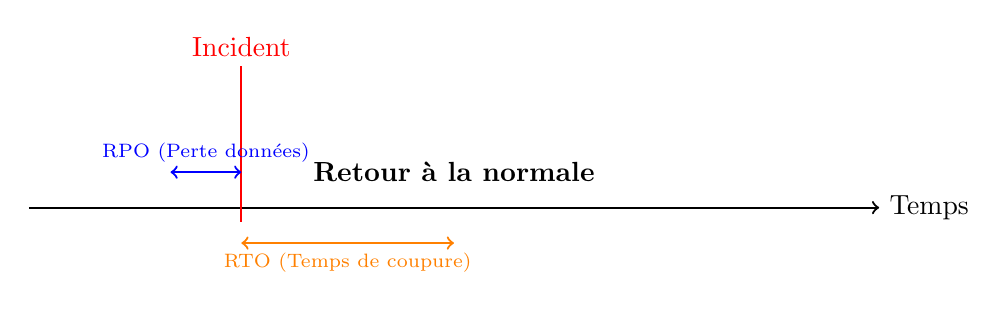
\begin{tikzpicture}[scale=0.9]
    % Axe du temps
    \draw[->, thick] (0,0) -- (12,0) node[right] {Temps};
    
    % Incident
    \draw[thick, red] (3,-0.2) -- (3,2);
    \node[above, red] at (3,2) {Incident};
    
    % RPO
    \draw[<->, thick, blue] (2,0.5) -- (3,0.5);
    \node[above, blue, font=\scriptsize] at (2.5,0.5) {RPO (Perte données)};
    
    % RTO
    \draw[<->, thick, orange] (3,-0.5) -- (6,-0.5);
    \node[below, orange, font=\scriptsize] at (4.5,-0.5) {RTO (Temps de coupure)};

    % Restauration
    \node at (6,0.5) {\textbf{Retour à la normale}};
\end{tikzpicture}
\caption{Schéma RTO vs RPO}
\end{figure}

\begin{boxlizbiz}
\textbf{Exemple LiZbiZ - Serveur ERP :}
\begin{itemize}
    \item \textbf{RTO = 4 heures :} Si l'ERP tombe, LiZbiZ doit le remettre en route en moins de 4h (sinon perturbation de la logistique).
    \item \textbf{RPO = 1 heure :} On ne peut pas perdre plus d'une heure de commandes clients.
    \textbf{Conséquence technique :} Les sauvegardes doivent être faites toutes les heures (RPO), et il faut un serveur de secours capable de démarrer rapidement (RTO).
\end{itemize}
\end{boxlizbiz}

% ------------------------------------------------------------------------------
\section{Les Stratégies de Reprise (PCA et PRA)}
% ------------------------------------------------------------------------------

\subsection{Distinction PCA / PRA}

Il ne faut pas confondre les deux plans :

\begin{itemize}
    \item \textbf{PCA (Plan de Continuité d'Activité) :} C'est le plan \textbf{Métier}. Comment l'entreprise continue de travailler si l'informatique est coupée ? (Ex: Traitement manuel des commandes, travail au papier).
    \item \textbf{PRA (Plan de Reprise d'Activité) :} C'est le plan \textbf{IT}. Comment restaurer les systèmes informatiques ? (Ex: Bascule sur un site de secours, restauration des sauvegardes).
\end{itemize}

Le PRA sert le PCA.

\subsection{Types de Sites de Secours (pour le PRA)}

Pour respecter le RTO, l'entreprise peut disposer de sites de secours :

\begin{enumerate}
    \item \textbf{Site Froid (Cold Site) :} Locaux vides, électricité et climatisation uniquement. Long à activer (semaines). Peu coûteux.
    \item \textbf{Site Tiède (Warm Site) :} Matériel présent mais éteint. Activation en jours.
    \item \textbf{Site Chaud (Hot Site) :} Matériel allumé et synchronisé en temps réel. Activation en heures (ou minutes). Très coûteux.
\end{enumerate}

% ------------------------------------------------------------------------------
\section{Cas LiZbiZ : Atelier BIA et Stratégie}
% ------------------------------------------------------------------------------

\subsection{Atelier : Définition des Besoins}

\begin{boxlizbiz}
\textbf{Scénario :} Un incendie s'est déclaré dans le local serveur principal de LiZbiZ. Toute l'infrastructure (Serveurs, ERP, Web) est détruite. Heureusement, le personnel est sain et sauf.
\end{boxlizbiz}

\textbf{Exercice de groupe :}

Pour les 3 processus suivants, définissez le RTO, le RPO et la stratégie de secours :

\begin{table}[htbp]
\centering
\small
\begin{tabular}{p{3cm}p{2cm}p{2cm}p{5cm}}
    \toprule
    \textbf{Processus} & \textbf{RTO} & \textbf{RPO} & \textbf{Stratégie Proposée} \\
    \midrule
    Site E-commerce (Vente) & 1h & 0 (Temps réel) & \textit{(A vous de jouer)} \\
    ERP (Gestion Stock) & 4h & 1h & \textit{(A vous de jouer)} \\
    Intranet RH & 1 semaine & 24h & \textit{(A vous de jouer)} \\
    \bottomrule
\end{tabular}
\end{table}

\textbf{Pistes de réflexion (Corrigé) :}
\begin{itemize}
    \item \textbf{Site Web (RTO 1h, RPO 0) :} Nécessite un Site Chaud ou une infrastructure Cloud (ex: AWS) avec réplication temps réel (Active-Active). Coût élevé mais vital pour le chiffre d'affaires.
    \item \textbf{ERP (RTO 4h, RPO 1h) :} Nécessite un Site Tiède (Warm Site) avec restauration de sauvegardes horaires. Compromis coût/performance.
    \item \textbf{Intranet RH :} Peut attendre. Site Froid ou simple restauration depuis des sauvegardes externes (tapes/Cloud froid) quand le reste est rétabli.
\end{itemize}

% ==============================================================================
% Fichier : 04_module_incident.tex (Extrait Chapitre 5)
% Description : Application Pratique - Mise en œuvre du PCA
% ==============================================================================